\documentclass{beamer}

\usepackage{focs-slides}
\usepackage{pifont}
\usepackage{xcolor}
\usepackage{pgf}
\usepackage{minted}
\usemintedstyle{perldoc}
\usepackage{lipsum}
\usepackage{enumerate}
\usepackage{hyperref}
\usepackage[font=scriptsize,labelfont=bf]{caption}
\captionsetup{labelfont={color=black}}


\definecolor{bg}{rgb}{0.95,0.95,0.95}
\setminted{
    %bgcolor=black,
    linenos,
    breaklines,
    fontsize=\footnotesize,
    tabsize=4
}
\setmintedinline{
    fontsize=\footnotesize
}
\newcommand{\LC}[1]{\mintinline{latex}{ #1 }}
\newcommand{\LCL}[1]{\begin{minted}{latex}{
#1
}\end{minted}}
\usepackage[utf8]{inputenc}
\usepackage{tcolorbox}
\tcbuselibrary{minted,skins}

\definecolor{bill}{RGB}{0,0,0}
\definecolor{numC}{RGB}{220,220,220}

\newtcblisting{mycode}{
    listing engine=minted,
    minted style=perldoc,
    minted language=python,
    minted options={fontsize=\small,linenos,numbersep=3mm},
    %colback=bill,
    %colframe=bill,
    listing only,
    left=5mm,
    enhanced,
    overlay={\begin{tcbclipinterior}\fill[numC](frame.south west)rectangle([xshift=5mm]frame.north west);\end{tcbclipinterior}}
}

\newtcblisting{bashcode}{
    listing engine=minted,
    minted style=perldoc,
    minted language=bash,
    minted options={fontsize=\small,linenos,numbersep=3mm},
    %colback=bill,
    %colframe=bill,
    listing only,
    left=5mm,
    enhanced,
    overlay={\begin{tcbclipinterior}\fill[numC](frame.south west)rectangle([xshift=5mm]frame.north west);\end{tcbclipinterior}}
}

\newtcblisting{bashcodetiny}{
    listing engine=minted,
    minted style=perldoc,
    minted language=bash,
    minted options={fontsize=\scriptsize,linenos,numbersep=3mm},
    %colback=bill,
    %colframe=bill,
    listing only,
    left=5mm,
    enhanced,
    overlay={\begin{tcbclipinterior}\fill[numC](frame.south west)rectangle([xshift=5mm]frame.north west);\end{tcbclipinterior}}
}

\newtcblisting{mycodetiny}{
    listing engine=minted,
    minted style=perldoc,
    minted language=python,
    minted options={fontsize=\scriptsize,linenos,numbersep=2mm},
    %colback=bill,
    %colframe=bill,
    listing only,
    left=5mm,
    enhanced,
    overlay={\begin{tcbclipinterior}\fill[numC](frame.south west)rectangle([xshift=5mm]frame.north west);\end{tcbclipinterior}}
}

\newtcblisting{mycodesql}{
    listing engine=minted,
    minted style=perldoc,
    minted language=sql,
    minted options={fontsize=\footnotesize,linenos,numbersep=3mm},
    %colback=bill,
    %colframe=bill,
    listing only,
    left=5mm,
    enhanced,
    overlay={\begin{tcbclipinterior}\fill[numC](frame.south west)rectangle([xshift=5mm]frame.north west);\end{tcbclipinterior}}
}

\usepackage{forest}
%\usepackage{ctex}
\title{Win or Lose?}
\author{Team \textsl{1} - Kezhi, Yinchen, Shaoze, Jiache}
\date{Summer 2023}
\course{ece472}

\definecolor{darkblue}{HTML}{6666dd} 
\definecolor{darkslategray}{HTML}{2f4f4f} 
\definecolor{yszqthree}{HTML}{6415ac}
%\colortheme{green!42!black}
%\colortheme{orange!85!black}
%\colortheme{darkblue}
%\colortheme{pink!80!black}
%\colortheme{orange!85!white!90!black}
\colortheme{darkslategray}
%\colortheme{yszqthree}


\begin{document}

\maketitle

% table of contents
\toc{enum}
% \toc{mindmap}




\section{Data Preparation}
\begin{frame}[fragile]
\frametitle{Mounting}
The following codes are added to \mintinline{bash}{~/.bashrc} to automatically mount millionsongs upon booting.
\begin{bashcode}
echo "password" | sudo -S sshfs /home/hadoopuser/ece472 -o allow_other -o Port=2223 ece472@focs.ji.sjtu.edu.cn: -o IdentityFile=~/.ssh/id_ed25519 1>/dev/null 2>/dev/null
echo "password" | sudo -S mount /home/hadoopuser/ece472/millionsong.iso /home/hadoopuser/ece472/ 1>/dev/null 2>/dev/null
\end{bashcode}
\end{frame}

\begin{frame}[fragile]
\frametitle{H5 Files}


\begin{minipage}{0.5\linewidth}
\begin{forest}
for tree={
  font=\ttfamily,
  grow'=0,
  child anchor=west,
  parent anchor=south,
  anchor=west,
  calign=first,
  edge path={
    \noexpand\path [draw, \forestoption{edge}]
    (!u.south west) +(7.5pt,0) |- (.child anchor) pic {folder} \forestoption{edge label};
  },
  before typesetting nodes={
    if n=1
      {insert before={[,phantom]}}
      {}
  },
  fit=band,
  before computing xy={l=15pt},
}
[Track.h5
  [analysis
    [bars confidence]
    [...]
  ]
  [metadata
    [artist terms]
    [...]
  ]
  [musicbrainz
    [artist mbtags]
    [...]
  ]
]
\end{forest}
\end{minipage}
\begin{minipage}{0.4\linewidth}
\begin{itemize}
    \item We used \textbf{python h5py} module to extract information in \textit{.h5} files.
    \item We collect useful fields in all \textit{.h5} files and summarize them in one single \textit{.avro} file
\end{itemize}
\end{minipage}
\end{frame}

\begin{frame}[fragile]
\frametitle{avro File}
    \begin{itemize}
        \item Divide the dataset into 26 parts
        \item Create one \textit{.avro} file for all files in each part
        \item Use \textbf{pyspark} to parallelize the process
        \item Merge 26 small \textit{.avro} files into one single big file
    \end{itemize}
    \vspace{0.5cm}
    With 8 cores processing in parallel, the total time cost to form one \textit{.avro} file is reduced from 6 hours to 3 hours.
    
    \vspace{0.2cm}
    
    The \textit{.avro} file generated which is consisted of all desired features of one million songs is approximately 150Mb.
\end{frame}

\begin{frame}{EDA}


\begin{table}[htbp]
\captionsetup{font=small}
  \centering
  \caption{Statistic of Raw Data}
    \begin{tabular}{rrrrrr}
          & \multicolumn{1}{l}{\textbf{tempo}} & \multicolumn{1}{l}{\textbf{hotness}} & \multicolumn{1}{l}{\textbf{year}} & \multicolumn{1}{l}{\textbf{time\_signature}} & \multicolumn{1}{l}{\textbf{...}}\\
    \midrule
    \textbf{count} & 1000000 & {\color{red} 581965} & 1000000 & 1000000 & \\
    \textbf{mean} & 123.889 & 0.356 & {\color{red}1030}  & 3.59 &\\
    \textbf{std} & 35.056 & 0.234 & 999   & 1.22 &\\
    \textbf{min} & 0.000 & 0.000 & 0     & 0 &\\
    \textbf{25\%} & 97.995 & 0.215 & 0     & 3 &\\
    \textbf{50\%} & 122.086 & 0.378 & 1969  & 4 &\\
    \textbf{75\%} & 144.089 & 0.532 & 2002  & 4 &\\
    \textbf{max} & 302.300 & 1.000 & 2011  & 7 &\\
    \end{tabular}%
  \label{tab:addlabel}%
  
\end{table}%



\end{frame}


\begin{frame}{Feature Analysis}
What features are needed to describe a Song?

\begin{enumerate}
    \item \textrm{Duration}
    \begin{itemize}
        \item The duration cannot directly determine the style of songs
        \item Adjusting granularity \& OneHotEncoder
        
    \end{itemize}

    \item \textrm{Segments\_loudness\_max / Segments\_loudness\_max\_time}
    \begin{itemize}
        \item The most load segment can be regarded as the \textbf{"musical climax"}
        \item Classify this feature by the occurrence of musical climax. 
    \end{itemize}

    \item \textrm{Segments\_pitches}
    \begin{itemize}
        \item Analyze \textbf{emotion} of song by computing the mean of pitches.
        \item Associate with the \textrm{Segments\_loudness\_max} 
    \end{itemize}
    
\end{enumerate}


\end{frame}



\begin{frame}{Feature Engineering}
\begin{columns}
    \column{0.5\textwidth}
    \textbf{Prepare the data for Model:}
    \bigskip
    \begin{itemize}
    \item Missing \& Abnormal Value
    \item Distribution (Left/Right Skew)
    \item Granularity (Year)
    \item Encoding (One-hot, Hash...)
    \item Combination
    \item Normalize \& Standardize
    \end{itemize}

    \column{0.5\textwidth}
	\begin{figure}
		\centering
		% Requires \usepackage{graphicx}
		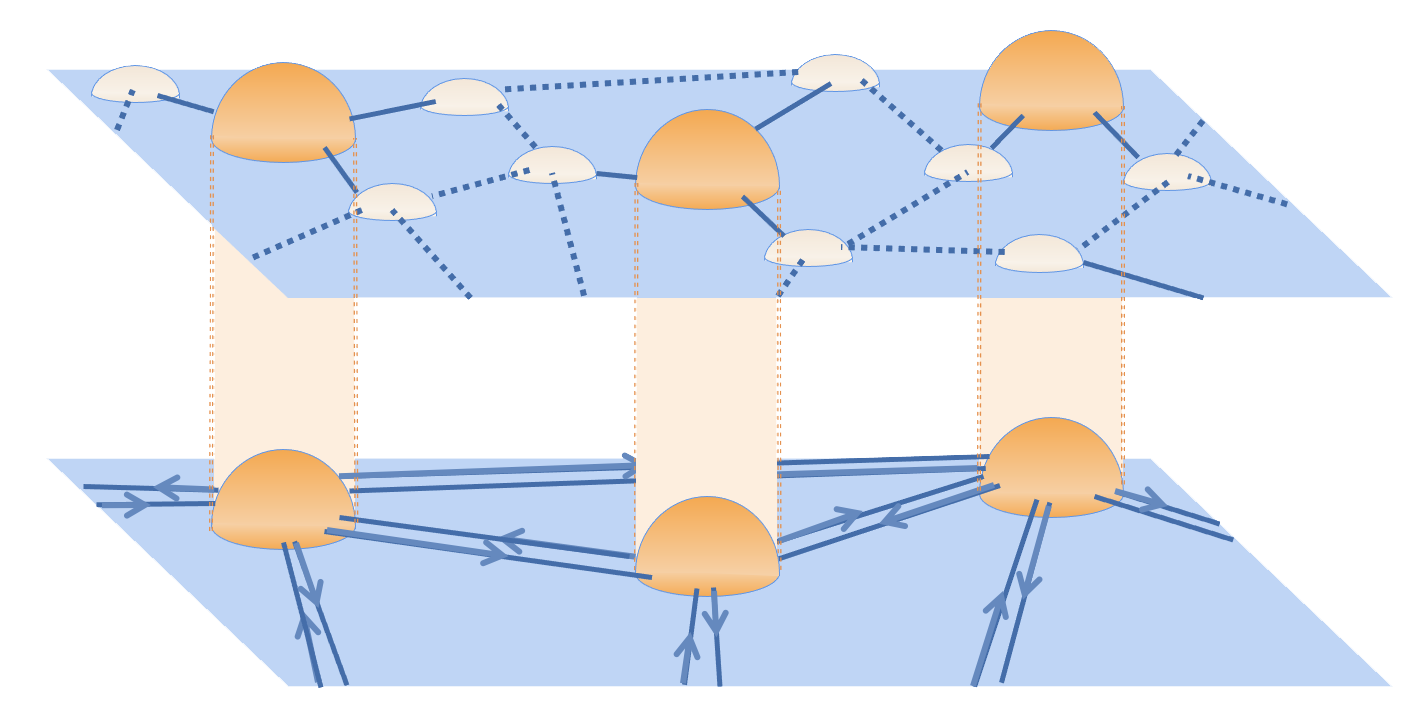
\includegraphics[width=5cm]{img/Feature_engineer.png}
		% \caption{secret sharing scheme}
		% \label{secert_sharing_figures}
	\end{figure}
\end{columns}
\end{frame}



\begin{frame}{Example: Loudness}

\begin{columns}
    \column{0.5\textwidth}
    \textbf{Issues:}
    \begin{itemize}
        \item Mostly $<0$ with $359/1000000$ abnormal values 
        \item Left skewed
    \end{itemize}
    \medskip
    \begin{figure}
		\centering
		% Requires \usepackage{graphicx}
		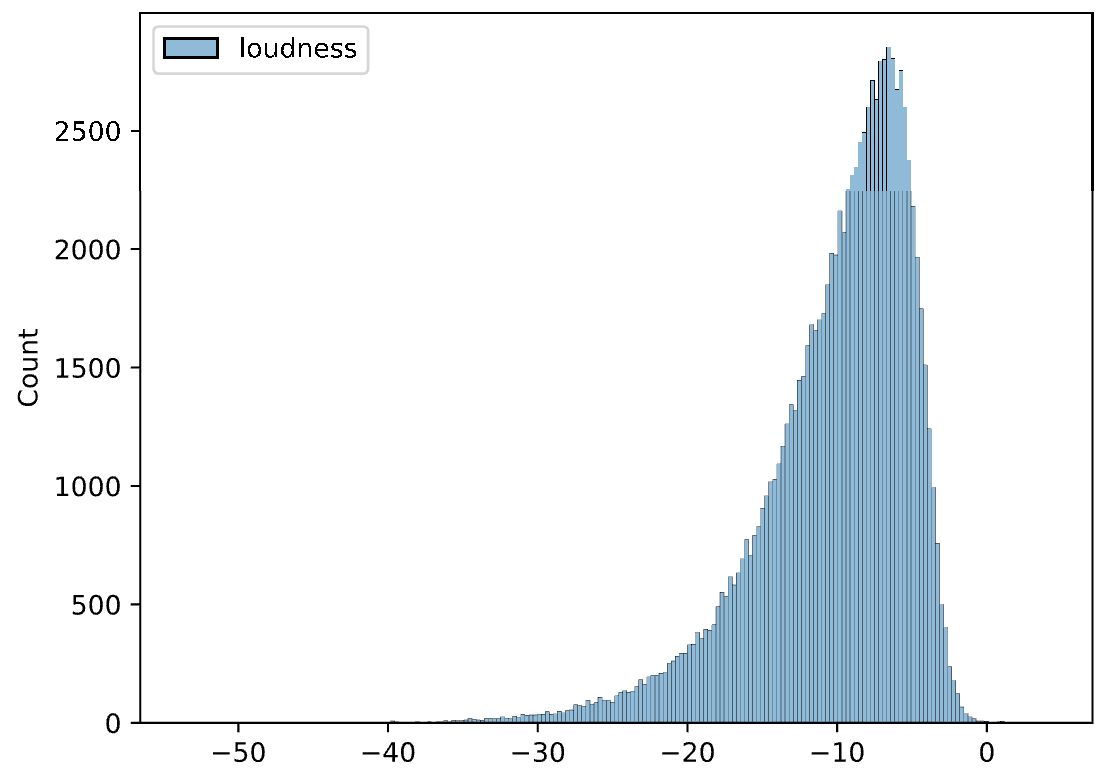
\includegraphics[width=5cm]{img/Loudness_before.png}
		\caption{Distribution of Raw Data}
		% \label{secert_sharing_figures}
    \end{figure}


    \column{0.5\textwidth}

    \textbf{Methods: }
    \begin{itemize}
        \item Replace exceptions with median 
        \item $loudness\_log = ln(- loudness)$
    \end{itemize}
    
	\begin{figure}
		\centering
		% Requires \usepackage{graphicx}
		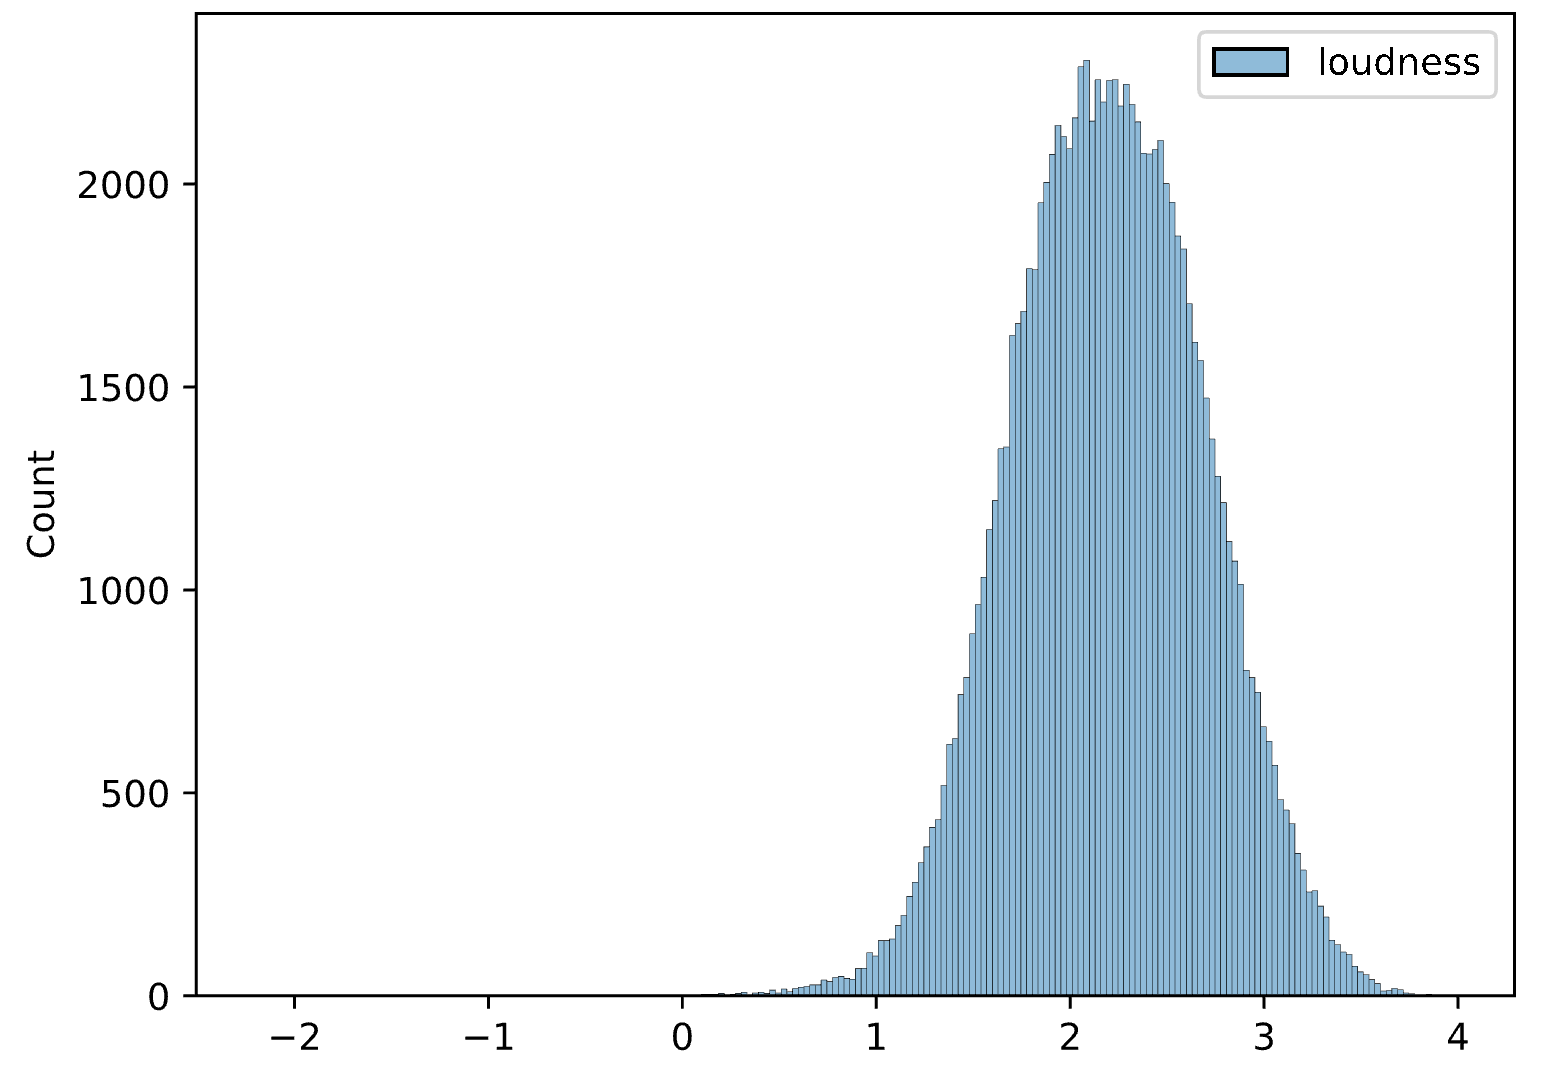
\includegraphics[width=5cm]{img/Loudness_after.png}
		\caption{Distribution of Adjusted Data}
		% \label{secert_sharing_figures}
	\end{figure}
\end{columns}










\end{frame}



\begin{frame}[fragile]{Pipeline}
\begin{mycodetiny}
processed_data = process_data_gm(data, (
    # Customized Column Transformer
    (log_transform_negative_column, ['loudness'], None),
    (classify_year_column, ['year'], None),
    (proportion_fade_out, None, None),
    (fade_out_time, None, None),

    # Exception Handling
    (drop_zeros, [List_of_Features], None),
    (fill_hotness_na_with_0, None,  None),

    # Normalize Selected Features
    (normalized_selected_columns, [List_of_Features], None),

    # Select Features
    (select_columns, ['Log_loudness', 'bar_num', 'beat_num', 
                      # Add features here
                      ], None),
))
\end{mycodetiny}  

    
\end{frame}





\section{Drill Database Query}

\begin{frame}
\frametitle{Motivation}
In this part, we used drill to perform simple database queries, including:

\begin{itemize}
    \item Find the range of dates covered by the songs in the dataset, i.e. the age of the \emph{oldest} and of the \emph{youngest} songs
    \item Find the \emph{hottest} song that is the \emph{shortest} and has the \emph{highest energy} with the \emph{lowest tempo}.
    \item Find the name of the album with the \emph{most tracks}.
    \item Find the name of the band(artists) who recorded the \emph{longest song}.
\end{itemize}
\end{frame}

\begin{frame}[fragile]

\frametitle{Preparation}

Given the avro file, we first created a table in drill

\begin{mycodesql}
-- read avro file from local file system (~100M)
create table dfs.tmp.`songs` as
select * from dfs.`F:/avro/songs.avro`;
-- change path
use dfs.tmp;
\end{mycodesql}

\end{frame}

\begin{frame}[fragile]
\frametitle{Detailed Solutions}

1. the oldest and youngest songs

\begin{mycodesql}
select max(year_end) from songs where year_end > 0;
+--------+ 
| EXPR 0 |
+--------+
| 2011   |
+--------+                                                                      
1 row selected (0.321 seconds)

select min(year_end) from songs where year_end > 0;              
+--------+
| EXPR 0 |
+--------+
| 1922   |
+--------+
1 row selected (0.323 seconds)
\end{mycodesql}


Therefore, the dataset covered songs from $1922$ to $2011$, namely the age of the songs vary from $12$ years to $101$ years.
\end{frame}

\begin{frame}[fragile]
    \frametitle{Detailed Solusions}

2. the hottest, shortest, highest energy, lowest tempo

\begin{mycodesql}
select id, title from songs 
where hotness <> 'NaN'
order by hotness desc, duration asc, energy desc, tempo asc
limit 5;

+--------------------+-----------------------------------+
|         id         |               title               | 
+--------------------+-----------------------------------+
| SONASKH12A58A77831 | Jingle Bell Rock                  |
| SOAVJBU12AAF3B370C | Rockin Around The Christmas Tree  |
| SOEWAKD12AB01860D5 | Holiday                           |
| SOAAXAK12A8C13C030 | Immigrant Song (Album Version)    |
| SOAXLDX12AC468DE36 | La Tablada                        |
+--------------------+-----------------------------------+
5 rows selected (0.497 seconds) 
\end{mycodesql}

Therefore, \verb|Jingle Bell Rock| is the song the hottest song that is the shortest and shows highest energy with lowest tempo.

\end{frame}

\begin{frame}[fragile]

\frametitle{Detailed Solutions}
3. the album with the most songs

\begin{mycodesql}
select album_id, album_name, count(album_id) as numSongs
from songs
group by album_id, album_name
order by numSongs desc
limit 1;

+----------+------------------------------------+----------+
| album_id |              album_name            | numSongs |
+----------+------------------------------------+----------+
| 60509    | First Time In A Long Time:         | 85       | 
|          | The Reprise Recordings             |          |
+----------+------------------------------------+----------+
1 row selected (1.076 seconds) 
\end{mycodesql}

\href{https://www.discogs.com/release/4483625-Fanny-First-Time-In-A-Long-Time-The-Reprise-Recordings}{First Time In A Long Time: The Reprise Recordings} is the album with most tracks. Indeed, it has 4CDs and 80+ tracks.
\end{frame}

\begin{frame}[fragile]
    \frametitle{Detailed Solutions}

    4. the band with longest song

\begin{mycodesql}
select artist_name, title, duration from songs
order by duration desc limit 1; 

+--------------------------------+------------+-----------+
|          artist_name           |   title    | duration  |
+--------------------------------+------------+-----------+ 
| Mystic Revelation of Rastafari | Grounation | 3034.9058 | 
+--------------------------------+------------+-----------+  
1 row selected (0.468 seconds) 
\end{mycodesql}

Therefore, the band \verb|Mystic Revelation of Rastafari| has recorded \verb|Grounation| which has highest duration.

\end{frame}

\section{Big Data Recommendation}



\begin{frame}
\frametitle{Similarity Metrics}
Similarity between $Song_A = [a_1, a_2, ..., a_n]$ and $Song_B = [b_1, b_2, ..., b_n]$

\begin{enumerate}
    \item {$L_1$ Norm} 
    
    $$
    d_{L_1} = \sum_{i=1}^{n} |a_i - b_i|
    $$
    
    \item Cosine Similarity 
    
    $$
    cos\theta = \frac{\sum_{i=1}^{n} (a_i \times b_i)}{\sqrt{\sum_{i=1}^n a_i^2} \times \sqrt{\sum_{i=1}^n b_i^2}}
    $$


    \item Combination
    
    $$
    Similarity(Song_A, Song_B) =  \lambda cos\theta - d_{L2}
    $$

    
\end{enumerate}
    
\end{frame}

\begin{frame}{Similar Artists based BFS}
\captionsetup{textfont={color=black}}
\begin{figure}
    \centering
    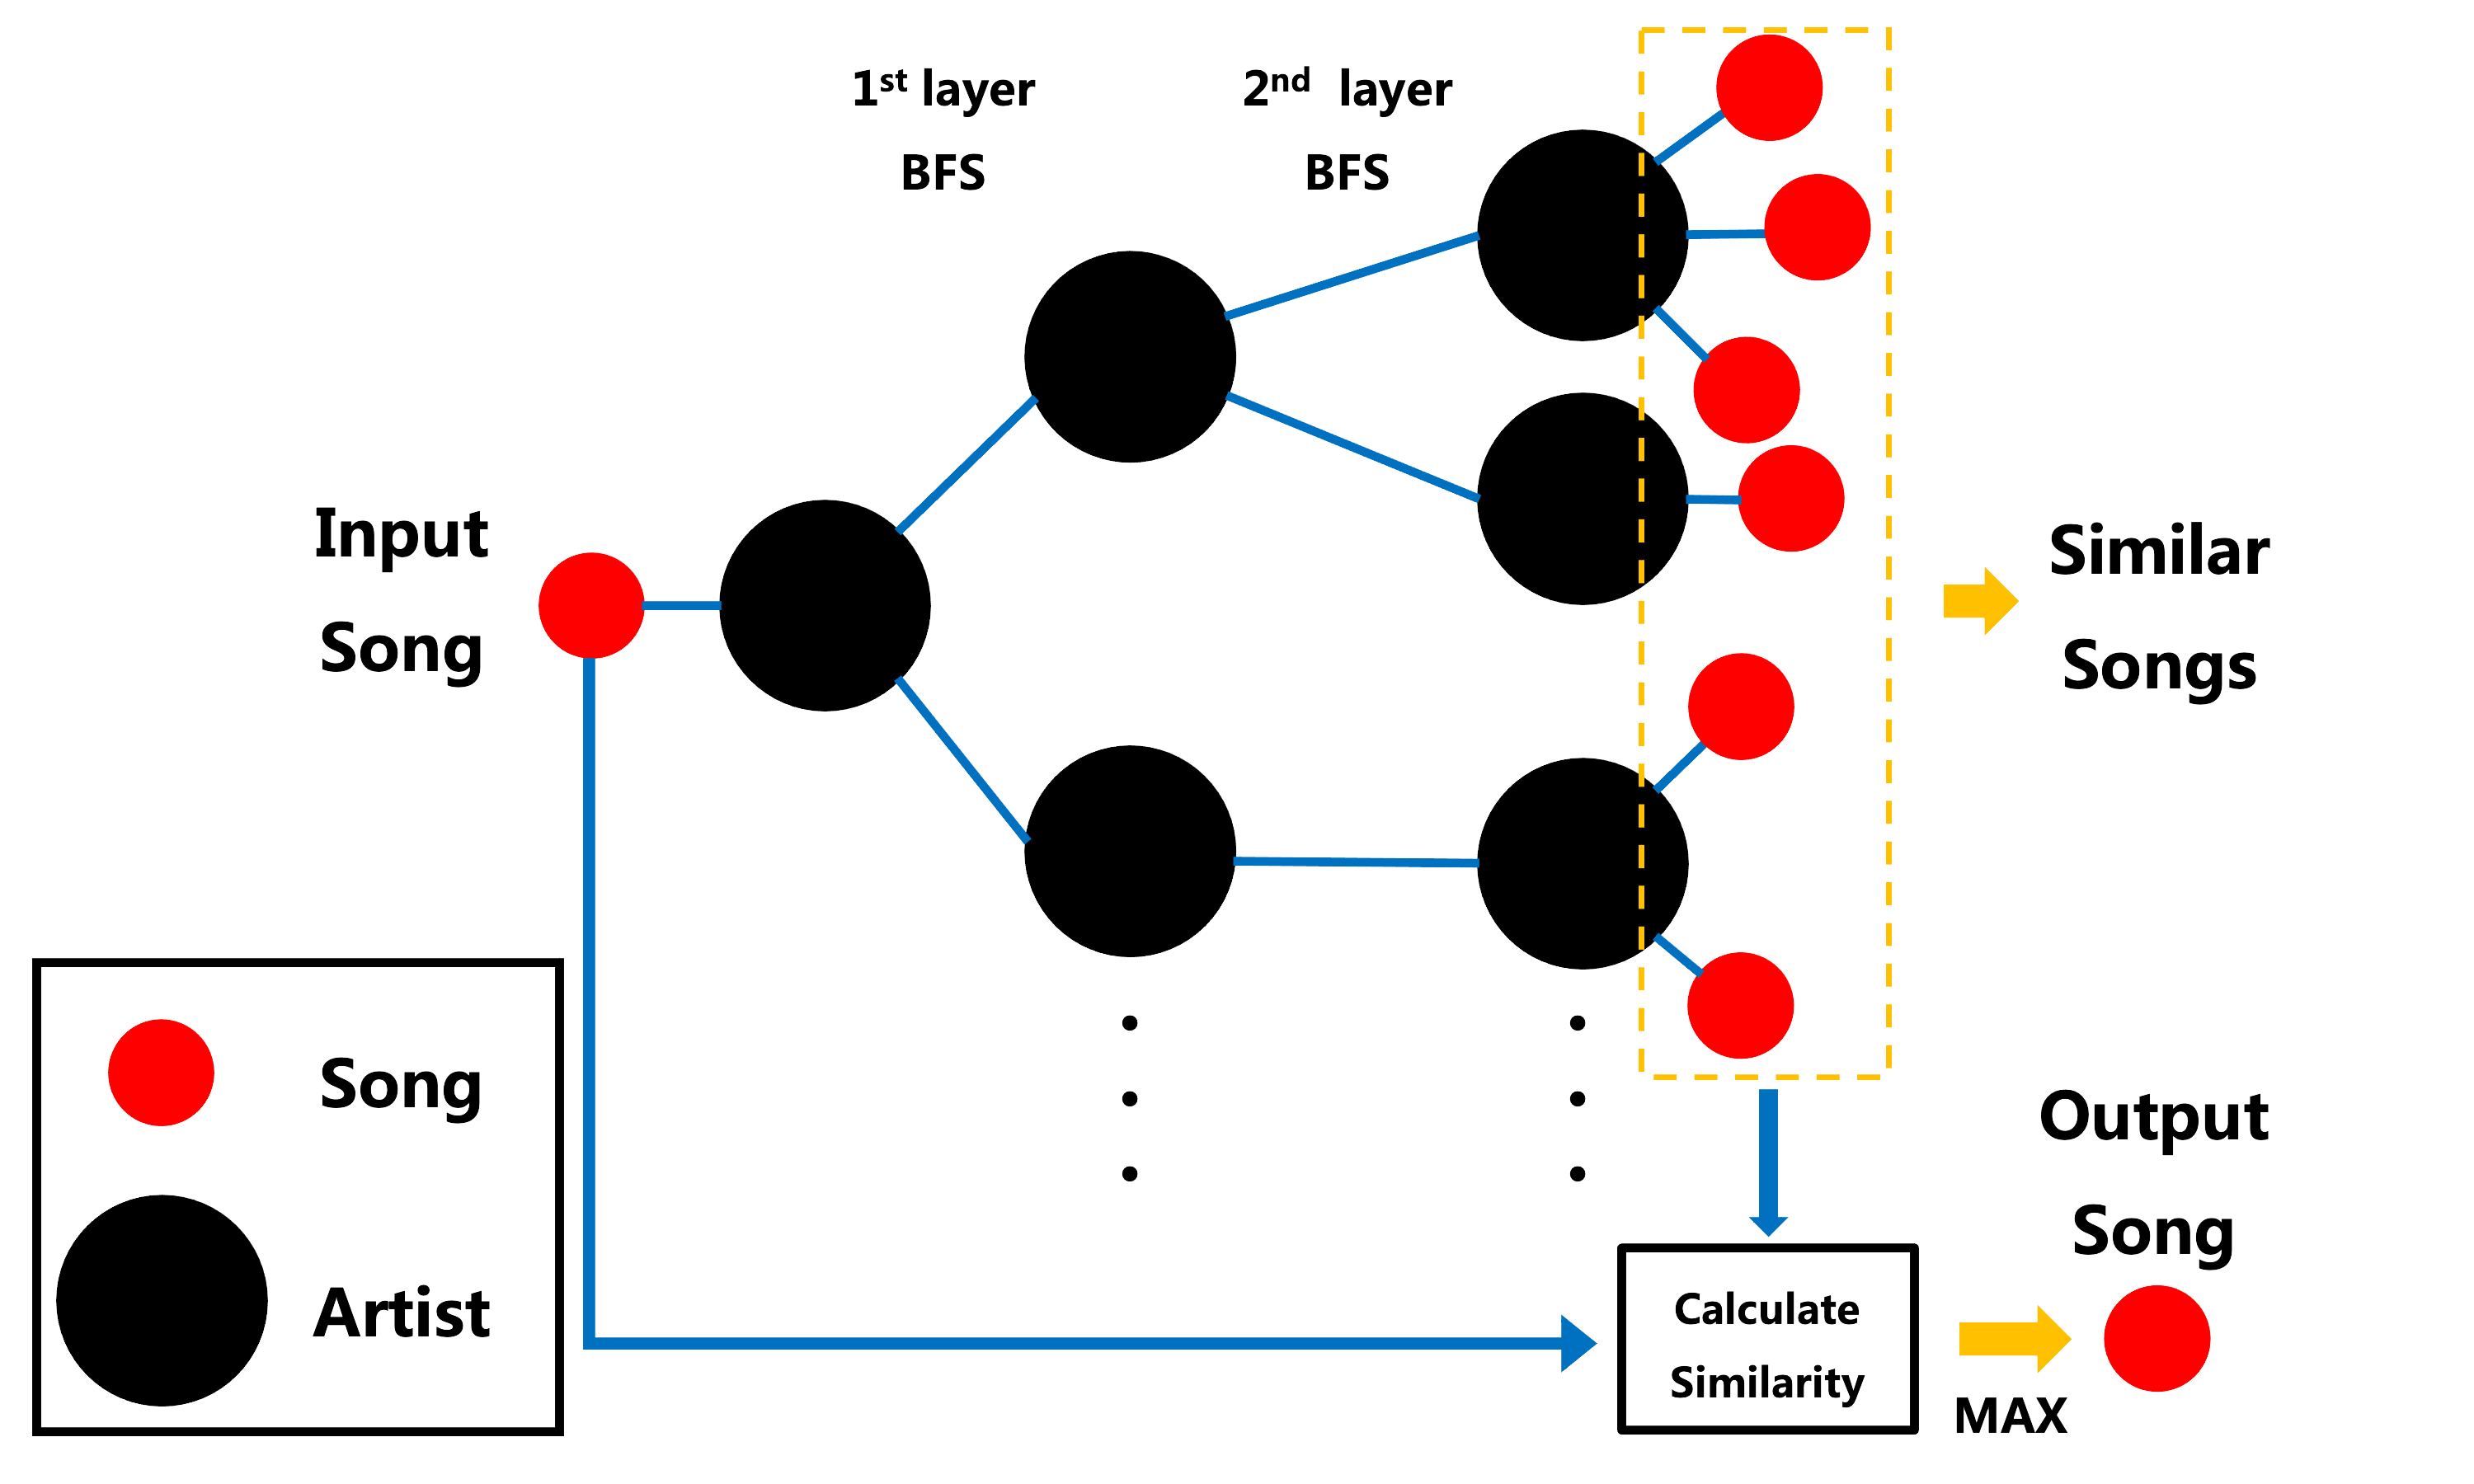
\includegraphics[width=0.9\linewidth]{img/bfs.png}
    \caption{Two layers BFS}
    \label{fig:bfs}
\end{figure}

\end{frame}


\begin{frame}{Example}
    \textbf{Input song:} (\href{https://music.163.com/#/song?id=1328484856}{Old Man Mose}, The Bristols)

    \bigskip
    \textbf{Recommended Song:}
    \begin{enumerate}
        \item $L_1$ Norm: (\href{https://music.163.com/#/song?id=553931121}{The Story of Two}, Micragirls)
        \item Cosine Similarity: (\href{https://music.163.com/#/song?id=1880855685}{Kentish (demo)}, Modwheelmood) 
        \item Combination:

        When $\lambda \leq 307$, (Kentish (demo), Modwheelmood).

        When $\lambda \geq 308$, (The Story of Two, Micragirls).
        
    \end{enumerate}
\vspace{0.35cm}
\end{frame}

\begin{frame}[fragile]

\frametitle{Diverse Recommendation Implementation}
\textit{Choose different $\lambda$ to reach diverse recommendations!}
\begin{mycodetiny}
import numpy as np
from numpy import ndarray
def calcDistance(song1: tuple, song2: ndarray) -> float:
    # song1: (feature: ndarray, track_Id: str)
    weight = 325
    return weight * (np.dot(song1[0], song2) / \ 
           (np.linalg.norm(song1[0]) * \ 
           np.linalg.norm(song2)) \ 
           - np.sum(np.abs(song1[0]-song2)), song1[1])

\end{mycodetiny}

\end{frame}


\begin{frame}{KMeans Recommendation}
\captionsetup{textfont={color=black}}
\begin{figure}
    \centering
    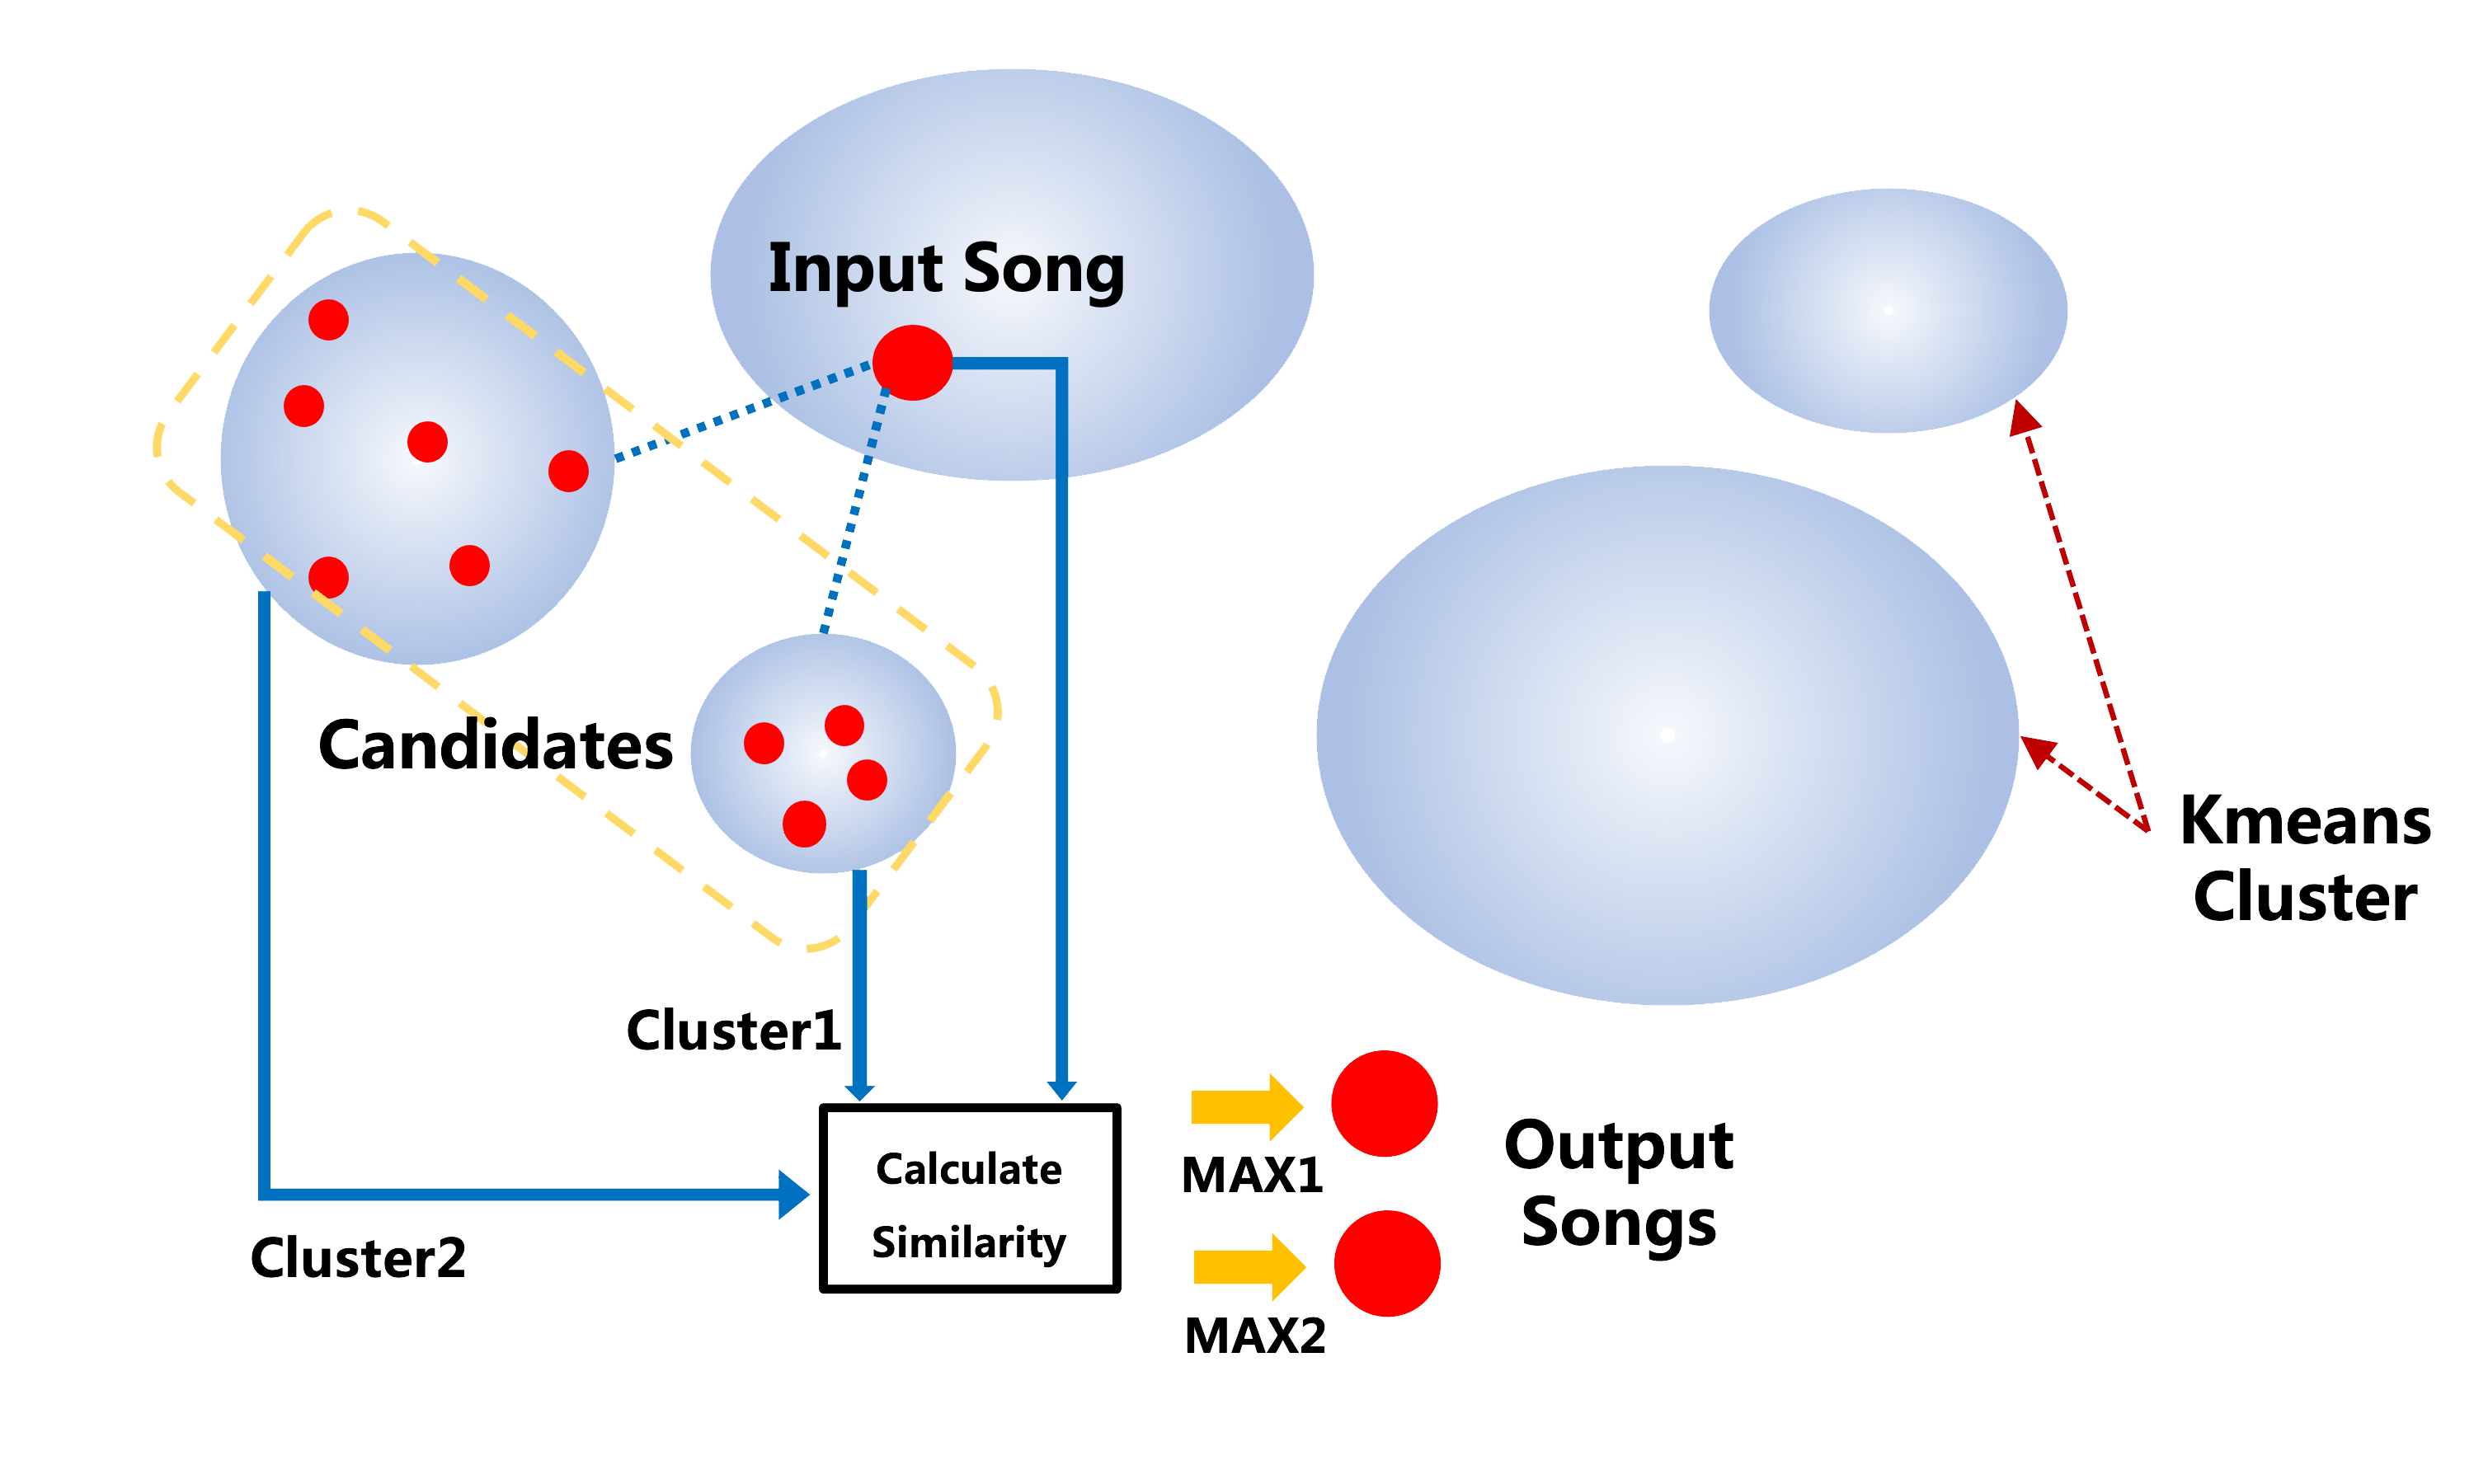
\includegraphics[width=0.9\linewidth]{img/Kmean.png}
    % \caption{Kmeans Recommendation}
    \label{fig:kmeans}
\end{figure}

\end{frame}

\begin{frame}[fragile]
\frametitle{KMeans Recommendation}
\begin{mycodetiny}
    def getKMostRelatedCenter(track_id, data, cluster_centers, k=3)-> list:

    song = data[data["track_id"] == track_id]
    song = song.loc[:, features_list].to_numpy()
    dis = []
    for center in cluster_centers:
        dis.append(np.dot(song, center) / (np.linalg.norm(song) * np.linalg.norm(center)))
    
    sorted_np = np.argsort(np.array(dis), axis=0)[:,0] < k
    index = range(0, np.shape(cluster_centers)[0])

    cluster_centers_withindex = np.hstack((cluster_centers, np.array(index).reshape(-1, 1)))
    selected_centers = cluster_centers_withindex[sorted_np][:, -1]
    return list(selected_centers)
    
\end{mycodetiny}

\end{frame}


\begin{frame}{Example}
    \textbf{Input song:} (\href{https://music.163.com/#/song?id=1328484856}{Old Man Mose}, The Bristols)
    \bigskip
    
    \textbf{Recommended Song:}
    \begin{enumerate}
        \item Cluster\_Center1: (\href{https://music.163.com/song?id=5193056&userid=1763329628}{Professor Ironside}, Lloyd Parks)
        \item Cluster\_Center2: (\href{https://music.163.com/song?id=537994085&userid=1763329628}{Por Telefono}, Los Nemus del Pacifico) 
        \item Cluster\_Center3: (\href{https://music.163.com/song?id=26714968&userid=1763329628}{Heaven Must Have Sent You}, The Elgins)
        
    \end{enumerate}
\vspace{0.35cm}
\end{frame}




\begin{frame}[fragile]

\frametitle{MapReduce Implementation}

Function of \verb|mapper|s and \verb|reducer|:
\begin{itemize}
    \item \verb|mapper_artist.py|: given an artist id as input, find all the similar artists (according to the database)
    \item \verb|mapper_song.py|: given the similar artists, find all of their songs
    \item \verb|mapper_distance.py|: given the list of songs, calculate their cosine similarity from the given song
    \item \verb|reducer.py|: find the song with largest similarity
\end{itemize}

    
\end{frame}

\begin{frame}[fragile]

\frametitle{MapReduce Performance}

We implement a \verb|driver.sh| to run the three map reduce job:

\begin{bashcode}
# How to run
cd MapReduce
time bash ./driver.sh
# Result
+ hdfs dfs -cat /project_distance/part-00000
('Story Of Two', 'TRMHEEB12903C9F3C9', 0.9140447260983122)

real    4m18.674s
user    1m27.983s
sys     0m5.830s
\end{bashcode}

\end{frame}

\begin{frame}[fragile]

\frametitle{Pyspark Implementation}

Use the same strategy, we implement the map and reduce in spark:
\begin{mycodetiny}
sc = SparkContext()
# find the list of similar artists
for i in range(depth):
    artists += sc.parallelize(artists, 4)\
               .map(artistNeighbor).reduce(merge_lists)
# find all the songs of similar artists 
songs: list = sc.parallelize(artists, 12)\ 
              .map(getArtistSongs).reduce(merge_lists)
# find the feature of the input song
features = sc.parallelize(features, 100)\
             .map(lambda x: (np.concatenate((x[1:2], x[3:-7]))\
             .astype(np.float64), (x[-6],x[-5],x[-1]))).collect()
# reduce to get the song with largest similarity
result = sc.parallelize(features, 100)\
           .map(lambda x: calcDistance(x, songFeature))\
           .reduce(lambda x, y: max(x, y))
\end{mycodetiny}
For pyspark, there is an interface for you to play with :).
\end{frame}

\begin{frame}[fragile]

\frametitle{Pyspark Performance}

\begin{bashcodetiny}
Please enter the name of a song:  Old Man Mose
Too many songs have the same name! Please choose a specific author from the list: 
['Jesse Fuller', 'George Lewis And His New Orleans Stompers', 'Louis Armstrong', 'Manhattan Transfer', 'Kenny Ball And His Jazzmen', 'The Bristols']
The author of your song: The Bristols
The song you choose: 
Name: Old Man Mose, Author: The Bristols, Id: TRYESJS12903CDF730
Please enter the depth of the BFS: 2
Num of similar artists in the 1th layer: 48.
Num of similar artists in the 2th layer: 1134.
Num of similar songs: 29818.
(0.9140447260983123, ("Story Of Two", "TRMHEEB12903C9F3C9", "The Micragirls"))

real    0m32.016s
user    0m2.668s
sys     0m2.587s
\end{bashcodetiny}

That is \textbf{8} times speed up than Mapreduce!
\end{frame}

\section{Year Prediction}


\begin{frame}[fragile]
\frametitle{Data Selecting}
We want to train a model to predict the year of a song with its features.
\begin{mycodesql}
SELECT COUNT(*) AS year_num FROM songs WHERE year<>0;
+----------+
| year_num |
+----------+
| 515576   |
+----------+
1 row selected (0.402 seconds)
\end{mycodesql}
Approximately half of the songs have years labeled. We use 80\% of them as training set and 20\% as validation set.
\end{frame}

\begin{frame}[fragile]
\frametitle{Data Prepossessing}

\begin{itemize}
    \item Years are grouped by every 5 neighboring years so that total number of classes is reduced from 88 to 18.
    \item Each feature is normalized to the range of $[0,1]$
    \item Very few data are missing (less than $1\%$). We just fill them as 0 and it would be not a big deal to the model.
\end{itemize}


\end{frame}
\begin{frame}[fragile]
\frametitle{PCA}
We fitted a PCA model on the training set, which keeps 6 principal components from 15 original features.
\begin{mycode}
pca = PCA(k=6, inputCol='features', outputCol='pca_features')
pca_model = pca.fit(feature_df)
return pca_model
pca_df = pca_model.transform(feature_df)
res_df =pca_df.select('coarse_classified_class_year',
'pca_features').rdd.map(lambda x: Row(tag=x[0],
PC1=float(x[1][0]), PC2=float(x[1][1]),
PC3=float(x[1][2]), PC4=float(x[1][3]),
PC5=float(x[1][4]), PC6=float(x[1][5])))
.toDF()
\end{mycode}
    
\end{frame}
\begin{frame}[fragile]
\frametitle{Model training}
We trained a logistic regression model to do the classification task.
\begin{mycode}
lrm = LogisticRegressionWithLBFGS.train(
sc.parallelize(data_train, 200), iterations=200, 
numClasses=18)
print("Weights:", lrm.weights)
lrm.save(sc,'file:///home/hadoopuser/project
             /predict/model')
\end{mycode}
\end{frame}
\begin{frame}[fragile]
\frametitle{Prediction results}
\begin{mycode}
(dfy['coarse_classified_class_year']==
 dfp['year_predict']).value_counts()
\end{mycode}
\begin{minipage}{0.49\linewidth}
\textbf{No PCA}
\begin{bashcode}
False    79282
True     23275
Name: count, 
dtype: int64
\end{bashcode}
\end{minipage}
\begin{minipage}{0.49\linewidth}
\textbf{Applying PCA}
\begin{bashcode}
False    71696
True     30861
Name: count, 
dtype: int64
\end{bashcode}
\end{minipage}

\vspace{0.2cm}

Applying PCA raises prediction accuracy from $22.69\%$ to $30.09\%$. For a 18 classification task, this result is satisfying enough.
\end{frame}


% \section{Final demostration}













% \begin{frame}{Sample frame}

% Bullet points:
% \begin{itemize}
% 	\item first element is in \R 
% 	\item second is in \C
% 	\item third is to show how to open and close ``quotes'' in \LaTeX
% \end{itemize}

% \medskip

% Numbered list:
% \begin{enumerate}
% 	\item first 
% 	\item second
% 	\item last but not least, only label equations that are reused
% \end{enumerate}

% \end{frame}



% \begin{frame}{Typesetting math content}
		
% \begin{theorem}
% 		If $\sigma$ and $\tau$ are two permutations of $\llbracket 1,n\rrbracket$, then $\varepsilon (\sigma\tau)=\varepsilon(\sigma)\varepsilon(\tau)$, and $\varepsilon$ is a group homomorphism from $\mathcal S_n$ to $(\{-1,1\},\times)$.
% \end{theorem}

% \begin{proof}
% 		For $A=(a_{i,j})_{1\le i,j\le n}$, $\det A$ is often denoted
% 		\[
% 			\det A = 
% 			\begin{vmatrix}
% 				a_{1,1} & \cdots & a_{1,j} & \cdots & a_{1,n}\\
% 				\vdots  &        & \vdots  &        & \vdots\\
% 				a_{i,1} & \cdots & a_{i,j} & \cdots & a_{i,n}\\
% 				\vdots  &        & \vdots  &        & \vdots\\
% 				a_{n,1} & \cdots & a_{n,j} & \cdots & a_{n,n}\\
% 			\end{vmatrix}.
% 		\]

% \end{proof}

% \end{frame}




% \begin{frame}{Include a picture}

% \begin{columns}[T,onlytextwidth]

% 	\column{.5\textwidth}
	
% 	\centering
% 	
\includegraphics[width=.7\columnwidth]{course}

% 	\column{.5\textwidth}

% 	\begin{example}
% 		Two columns aligned to the top with a picture on the left.
% 	\end{example}

% \end{columns}
		
% \end{frame}


\thankframe

\end{document}
